\documentclass[brudnopis]{xmgr}
\usepackage{amsrefs}
\usepackage{mathtools}
\usepackage{amsfonts}
\usepackage{ccaption}
\usepackage{amsthm}
\usepackage{todonotes}
\usepackage{placeins}
\usepackage{enumitem}

\DeclarePairedDelimiter\ceil{\lceil}{\rceil}
\DeclarePairedDelimiter\floor{\lfloor}{\rfloor}

\theoremstyle{definition}
\newtheorem{Twierdzenie}{Twierdzenie}
\newtheorem{Lemat}{Lemat} 
\newtheorem{Definicja}{Definicja} 

\wersja   {wersja wstępna [\ymdtoday]}

\author   {Jakub Ciechowski}
\nralbumu {186471}
\email    {jakubciechowski@gmail.com}

\title    {Problem galerii sztuki dla odcinków na płaszczyźnie}
\date     {\ymdtoday}
\miejsce  {Gdańsk}

\opiekun  {dr hab. Paweł Żyliński}

\begin{document}

\begin{abstract}
 W pierwszej częsci przedstawiam klasyczny problem galerii sztuki wraz z dowodem na minimalną liczbę strażników potrzebnych do strzeżenia wielokąta prostego o $n$ wierzchołkach oraz wielokąt o $h$ dziurach. W kolejnym rozdziale udowadniam ograniczenie górne oraz dolne dla strzeżenia oraz oświetlenia $n$ odcinków prostych na płaszczyźnie. Następnie, przedstawiam dowód problemu zbioru ukrytego w zbiorze $F$ rozłącznych odcinków. Kolejnym omówionym zagadnieniem są k-nadajniki dla których mając liczbę naturalną $k$ > 0 oraz dany obszar przedstawiam dowód dla wystarczającej oraz koniecznej liczby $1$-nadajników. W dalszej części rozdziału omawiam problem podziału gilotynowego wielokąta wraz z ograniczeniem górnym. Następnym zagadnieniem są siatki w dwóch oraz trzech wymiarach wraz z dowodem na minimalną ilość strażników w siatkach 2D oraz, że problem rozmieszczenia strażników w siatkach 3D należy do klasy problemów NP-zupełnych. Na koniec zajmuje się zagadnieniem problemu pościgu i ucieczki w grafie dowodząc, że w wariancie Sugiharu oraz Suzuki policjant jest w stanie zawsze zwyciężyć.
\end{abstract}
\keywords{Problem galerii sztuki, strzeżenie odcinków, problem iluminacji, k-nadajniki, strażnicy w siatkach, pościg i ucieczka w grafie}

\maketitle

\introduction
Jako pierwszy problem galerii sztuki przedstawił Victor Klee w 1973, odpowiadając na prośbę Vaseka Chv\'atala o interesujący problem geometryczny. Zagadnieniem, które zaproponował Klee było znalezienie minimalnej ilości strażników, wystarczających aby strzec wnętrze pomieszczenia galerii sztuki o kształcie $n$-kąta. Niedługo potem Chv\'atal zaproponował rozwiązanie tego problemu, które szybko zostało nazwane ,,Teorią galerii sztuki Chv\'atala''. Od tamtego dnia problem doczekał się wielu różnych wariacji oraz przekształceń. W pracy zajmę się rodziną problemów dotyczących odcinków na płaszczyźnie. 

Jednym z takich zagadnień jest strzeżenie zbioru odcinków, które wymaga aby strzeżony odcinek był widziany przez strażnika przynajmniej w jednym punkcie. Można to zobrazować przez stacjonarnych strażników, którzy, rozmieszczeni w odpowiednich punktach, zawsze widzą na przykład obraz, przez co uniemożliwiają zdjęcie go ze ściany. Innym ciekawym podejściem do sprawy strzeżenia odcinków jest ich oświetlanie, które  rozumiemy przez takie umieszczenie źródła światła aby każdy punkt należący do odcinka był widoczny z takiego źródła. Rozwiązaniem problemu jest zbiór źródeł światła które w całości oświetlają każdy odcinek należący do zbioru. 

Najbardziej nawiązującym do współczesności wariantem wywodzącym się z klasycznego problemu galerii sztuki jest problem k-nadajników. Traktuje on strażników jako nadajnik o nieskończonym zasięgu oraz określonej mocy. Mając dany zbiór przeszkód oraz znając moc nadajników (tzn. liczbę przeszkód przez którą nadajnik jest w stanie nadawać) rozwiązanie jest oszacowanie liczby nadajników pozwalających pokryć obszar, zawierający wszystkie przeszkody.

Kolejne zagadnienie wywodzące się z problemu galerii sztuki bazuje na zdegenerowanych wielokątach, a dokładnie na siatkach zarówno dwu jak i trójwymiarowych. Siatką nazywamy połączony ze sobą zbiór poziomych oraz pionowych odcinków prostych. Problem ten wymaga aby strażnik znajdował się w każdej z korytarzy siatki. Szacowanie liczby strażników dla siatek dwuwymiarowych ściśle wiąże się ze skojarzeniami w grafie natomiast dla siatek trójwymiarowych problem należy do klasy NP-zupełnej.

Ostatni rozdział łączy w sobie klasyczny problem galerii sztuki oraz elementy teorii grafów. Opisuje w nim wariant gry w policjanta i złodzieja, który wymaga aby policjant przemieszczający się z ograniczoną prędkością po krawędziach kraty zauważył złodzieja. Krata zdefiniowania jest podobnie jak siatka we wcześniejszym problemie. Zakładamy, że policjant widzi przez całą długość krawędzi.


\chapter{Podstawowe pojęcia}
W tym rozdziale znajdują się definicje postawowych pojęć wymaganych w dalszej części pracy.

\begin{Definicja}{Wielokąt prosty}

  Płaska figura składające się z $n$ wierzchołków $v_1, v_2,\ldots, v_n$ oraz $n$ krawędzi $v_1v_2, v_2v_3, \ldots, v_{n-1}v_n,v_nv_1$ takich, że żadna para kolejnych krawędzi nie przecina się.
\end{Definicja}

\begin{Definicja}{Graf prosty}

  Zbiór $G = (V,E)$, gdzie $V$ jest niepustym skończony zbiorem wierzchołków a $E$ jest skończonym zbiorem krawędzi.
\end{Definicja}

\begin{Definicja}{Graf spójny}

  Graf którego nie można przedstawić jako sumy dwóch grafów.
\end{Definicja}

\begin{Definicja}{Składowa spójności}
  
  \emph{Składową spójności} nazywamy spój podgraf grafu $G$ który nie należy do żadnego innego podgrafu spójnego.
\end{Definicja}

\begin{Definicja}{Skojarzenie}

  \emph{Skojarzeniem} w grafie $G$ nazywamy zbiór krawędzi $M$ takich, że każda krawędź z $G$ jest incydentna co najwyżej z jedną krawędzią z $M$. Najliczniejszym skojarzeniem nazywamy takie skojarzenie, które ma maksymalną moc.   
\end{Definicja}

\begin{Definicja}{Odcinek prosty}

  Część prostej łącząca dwa punkty.
\end{Definicja}

\begin{Definicja}{Strażnik}

  Punkt $p$ na płaszczyźnie, który \emph{strzeże} punktu $q$ wtedy i tylko wtedy jeżeli odcinek $\overline{pq}$ należy do wielokąta.
\end{Definicja}

\chapter{Klasyczny problem galerii sztuki}

\section{Twierdzenie Chv\'atala}\label{sec:klasyczny}
Zgodnie z twierdzeniem Chv\'atala \cite{chvatal} \label{tw chvatala}, minimalna liczba strażników potrzebnych do strzeżenia wielokąta prostego o $n$ wierzchołkach wynosi co najwyżej $\floor{\frac{n}{3}}$.
Z drugiej strony, istnieją $n$-kąty, które wymagają dokładnie $\floor{\frac{n}{3}}$.
\\\indent Przedstawię dowód Fiska \cite{fisk} powyższego twierdzenia, który jest znacznie prostszy od indukcyjnego dowodu Chv\'atala \cite{chvatal}, a bazuje na $3$-kolorowaniu odpowiedniego grafu triangulacji. 

Pierwszym krokiem jest triangulacja wielokąta $P$, przez dodanie wewnętrznych, nieprzecinających się przekątnych między wierzchołkami, do momentu gdy nie będzie można już dodać więcej przekątnych. 
Dowód na to, że każdy wielokąt prosty można podzielić na trójkąty, znajduje się w dodatku \ref{triangulacja}.
Za wierzchołki i krawędzie grafu triangulacji, przyjmujemy odpowiednio wierzchołki, krawędzie wielokąta oraz przekątne triangulacji. Jako że graf powstały po triangulacji jest planarny, zgodnie z twierdzeniem o czterech barwach \cite{appel} jest $4$-kolorowalny.

\begin{Definicja} 
   \emph{$K$-kolorowanie grafu} $G = (V,E)$ to przyporządkowanie takiej dodatniej liczby naturalnej każdemu wierzchołkowi grafu G, że żadnym dwóm sąsiednim wierzchołkom nie została przypisana taka sama liczba oraz wszystkie liczby są mniejsze bądź równe $K$.
\end{Definicja}

\begin{Lemat} \cite{fisk}
Graf triangulacji wielokąta prostego jest $3$-kolorowalny.
\end{Lemat}
\begin{proof}
	Dowód polega na indukcji po ilości trójkątów wielokąta po triangulacji. Trójkąt (graf $K_3$) jest przypadkiem bazowym -- zawsze można go pokolorować trzema kolorami. Następnym krokiem jest stworzenie grafu  dualnego dla grafu triangulacji danego wielokąta, który to jest drzewem. Grafem dualnym $G'$ nazywamy graf, który dla każdej ściany z grafu $G$ posiada odpowiadający jej wierzchołek połączony krawędzią z innym wierzchołkiem grafu $G'$ wtedy i tylko wtedy, gdy odpowiadające im ściany grafu $G$ są sąsiednie.
	\begin{figure}[ht!]
	  \centering
	  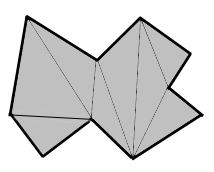
\includegraphics{rysunki/dual.png}
	    \caption{Wielokąt podzielony na trójkąty.}
	\end{figure} 
	Z grafu dualnego usuwamy dowolny liść wraz z odpowiadającym mu ,,trójkątem'', kolorujemy wierzchołki grafu triangulacji (z założenia indukcyjnego jest to możliwe), a następnie dodajemy trójkąt z powrotem nadając usuniętemu liściowi kolor inny niż używają jego dwaj sąsiedzi.
  \begin{figure}[ht!]
    \centering
      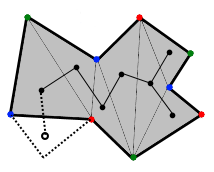
\includegraphics{rysunki/dual_kolor.png} 
      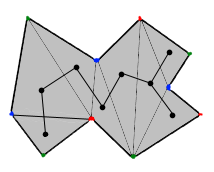
\includegraphics{rysunki/dual_caly_kolor.png}
      \caption{Pokolorowany graf triangulacji wraz z grafem dualnym.}
  \end{figure} 
\end{proof}
	Strażników rozmieszczamy w tych wierzchołkach, których kolor jest najrzadziej używanym.

\indent Ograniczenie ,,co najwyżej $\floor{\frac{n}{3}}$'' nie oznacza, że wystarczy rozmieścić strażnika w co trzecim wierzchołku -- patrzy rysunek niżej.
\begin{figure}[ht!]
  \centering
  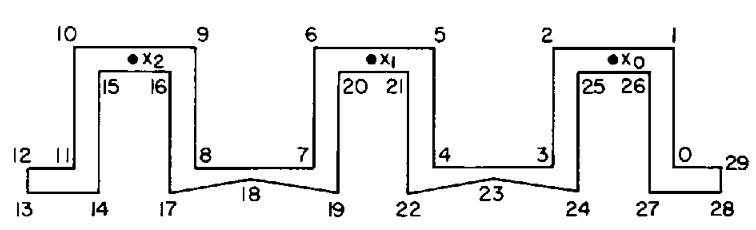
\includegraphics{rysunki/co_trzeci.png}
  \caption{Punkt $x$ jest niestrzeżony, przy rozmieszczeniu strażników w co trzecim wierzchołku.}
\end{figure} 

\section{Wielokąty z dziurami}
Ciekawym rozwinięciem klasycznego zagadnienia galerii sztuki jest wprowadzenie dziur do wnętrza wielokąta.

\begin{Definicja} \label{def wielokat z dziurami}
  \emph{Wielokątem z dziurami} nazywamy wielokąt P, który mieści w sobie wiele innych wielokątów $H_1, \ldots, H_n$ nazywanych \emph{dziurami}. Żaden wielokąt nie może przecinać zarówno krawędzi wielokąta $P$, jak i innych wielokątów wewnętrznych $H_i$.
\end{Definicja}

\indent Podobnie jak w przypadku standardowych wielokątów, również dla wariantu z dziurami, aby obliczyć potrzebną ilość strażników, wykorzystamy triangulację.

\begin{Lemat} \cite{orourke}
  Każdy wielokąt z dziurami można podzielić na trójkaty.
\end{Lemat}

\begin{Lemat}\label{t trójkątów triangulacja} \cite{orourke}
  Każdy wielokąt $P$ o $h$ dziurach oraz $n$ krawędziach poddany triangulacji dzieli się na $t = n + 2h - 2$ trójkątów.
\end{Lemat}

W dowodzie powyższego lematu skorzystam z twierdzenia Eulera.
\begin{Twierdzenie} \label{tw eulera} \cite{euler}
  Niech $G$ będzie spójnym grafem płaskim o $N$ wierzchołkach, $M$ krawędziach oraz $F$ ścianach. Wówczas $N - M + F = 2$.
\end{Twierdzenie}

\begin{proof}[Dowód lematu]
	Korzystając z twierdzenia Eulera mamy $N$ wierzchołków, $F = t + h + 1$ ścian (po jednej na każdy trójkąt oraz dziurę i ścianę zewnętrzną) oraz $E = \frac{3t+n}{2}$ krawędzi (trzy krawędzie na każdy trójkąt plus krawędzie zewnętrzne liczone podwójnie).  Wówczas $V - E + F = 2$, a więc $n - \frac{3t+n}{2} + t + h + 1 = 2$, z czego wynika, że $t = n + 2h - 2$.
\end{proof}
Wiedząc, na ile trójkątów został podzielony wielokąt $P$, możemy przejść do twierdzenia oszacowującego wymaganą liczbę strażników.

\begin{Twierdzenie} \cite{orourke} \label{dominacjatriangulacji}
  Dla wielokąta o $n$ wierzchołkach oraz $h$ dziurach $\floor{\frac{n+2h}{3}}$ = $\ceil{\frac{t}{3}}$ strażników kombinatorycznych jest wystarczających, aby dominować każdą triangulację wielokąta.
\end{Twierdzenie}

Przez dominację rozumiemy zbiór strażników $C = {g_1,\ldots,g_k}$ taki, że przynajmniej w jednym wierzchołku każdego trójkąta grafu triangulacji znajduje się strażnik $g_i \in C$ \cite{orourke}. 
\\\indent Główną ideą dowodu jest kolejne usuwanie dziur wielokąta, wzdłuż przekątnych dodanych podczas triangulacji, poprzez łączenie ich ze ścianą zewnętrzną. Każda z dziur posiada krawędź w grafie triangulacji $T$, która łączy ją z inną dziurą lub z zewnętrzną krawędzią wielokąta $P$. ,,Przecięcie'' wzdłuż takiej krawędzi połączy dziurę ze ścianą zewnętrzną lub scali dwie dziury w jedną. W każdym z tych przypadków całkowita ilość dziur zmniejszy się o jeden. Trudność polega jedynie na wyborze krawędzi z $T$, które pozwolą uzyskać taki podział, że otrzymany wielokąt jest spójny.

\indent Niech $T'$ będzie grafem dualnym triangulacji (rysunek \ref{fig:triangulacja}). $T'$ jest grafem planarnym, stopnia co najwyżej trzy, posiadającym $h$ graniczących ze sobą skończonych ścian $F_1, \ldots, F_h$, po jednej na każdą dziurę wielokąta $P$. Niech $F_0$ będzie ścianą zewnętrzną. Wybieramy dowolną ścianę $F_i$, która posiada przynajmniej jedną wspólną krawędź $e$ ze ścianą $F_0$. Taka krawędź istnieje, ponieważ w grafie $T$ musi istnieć przekątna łącząca krawędź zewnętrzną wielokąta $P$ z jakąś dziurą -- w grafie $T'$ jest to krawędź $e$. Usunięcie krawędzi $e$ z $T'$ scala $F_i$ z $F_0$, bez rozspójniania grafu.

\begin{figure}[h!]
  \centering
    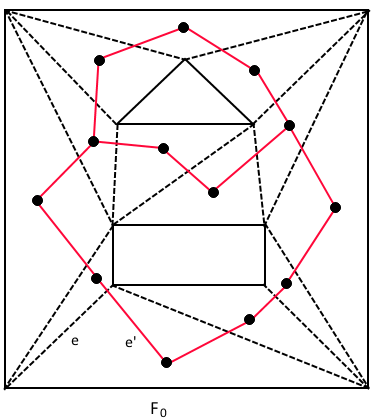
\includegraphics{rysunki/triangulacja_dziury.png}
    \caption{Wielokąt z dziurami wraz z grafem dualnym. Krawędź $e$ odpowiada krawędzi $e'$ w grafie dualnym.}
    \label{fig:triangulacja}
    \vspace{4in}
\end{figure} 

\indent Niech $P'$ będzie grafem triangulacji uzyskanym według powyższej procedury. W takim wypadku $P'$ posiada $n + 2h$ krawędzi oraz $t$ trójkątów, ponieważ każde cięcie daje nam dwie dodatkowe krawędzie, ale nie dodaje nowych trójkątów. Zgodnie z twierdzeniem \ref{dominacjatriangulacji}, $P'$ potrzebuje co najwyżej $\floor{\frac{n+2h}{3}} = \ceil{\frac{t}{3}}$ strażników.

\chapter{Strzeżenie zbioru odcinków}
\section{Strzeżenie zbioru odcinków prostych}\label{sec:strzezenie odcinkow}
Ten wariant zagadnienia galerii sztuki wymaga, aby strzeżony odcinek był widoczny przez strażnika przynajmniej w jednym punkcie. 
\begin{Definicja}
Niech $F = \{S_1,\ldots,S_n\}$ będzie zbiorem $n$ prostych odcinków na płaszczyźnie. Zbiór punktów $Q = \{p_1,\ldots,p_k\}$ \emph{strzeże} $F$, jeżeli każdy element $S_i$ ze zbioru $F$ zawiera punkt, który jest widziany przez przynajmniej jeden punkt $p_j$ należący do $Q$.
\end{Definicja}
Tak zdefiniowany problem możemy zobrazować przez strażników, którzy strzegą obrazu, jeżeli widzą tylko jego fragment. W takim przypadku nie można zdjąć obrazu ze ściany bez zaalarmowania strażnika.
\begin{figure}[ht!]
 \centering
  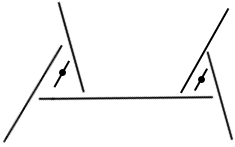
\includegraphics{rysunki/rozlaczny_dwoch_straznikow.png}
  \caption{Zbiór rozłącznych odcinków wymagający dwóch strażników.}
\end{figure} 

\begin{Twierdzenie} \label{straznicy strzezenie} \cite{illumination}
Aby \emph{strzec} dowolny zbiór $n$ rozłącznych odcinków prostych czasami potrzeba $\floor{\frac{2n-3}{5}}$, a zawsze wystarcza $\ceil{\frac{n}{2}}$ strażników.
\end{Twierdzenie}

\subsection{Ograniczenie górne}
Rozpatrzmy zbiór $F =\{S_1,\ldots,S_n\}$ rozłącznych odcinków prostych na płaszczyźnie oraz graf $G(F)$ zawierający $n$ wierzchołków $v_1$,\ldots,$v_n$ takich, że $v_i$ jest sąsiedni z $v_j$ wtedy i tylko wtedy, gdy istnieje punkt $x$ na płaszczyźnie, który widzi przynajmniej jeden punkt na odcinku $S_i$ i $S_j$ tzn. $x$ strzeże oba odcinki $S_i$ oraz $S_j$ (rysunek \ref{fig:zbior odcinkow rozlacznych}).

Aby udowodnić twierdzenie \ref{straznicy strzezenie} na początku wykażemy, że dla każdego zbioru $F$ rozłącznych odcinków prostych, których jest parzysta liczba $n$, odpowiednio zdefiniowany graf $G(F)$ ma doskonałe skojarzenie.

\begin{figure}[ht!]
 \centering
  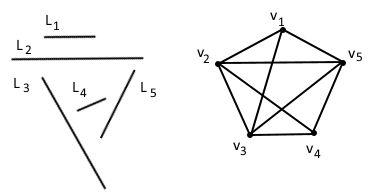
\includegraphics{rysunki/g_f.png}
  \caption{Zbiór $F$ rozłącznych odcinków oraz odpowiadający mu graf $G(F)$.}
  \label{fig:zbior odcinkow rozlacznych}
\end{figure} 

Mamy następujący lemat.
\begin{Lemat}\label{podgraf indukowany} \cite{illumination}
Niech $Q$ będzie dowolnym wielokątem prostym, a $F = \{S_1,\ldots,S_n\}$ zbiorem $n$ rozłącznych odcinków. Niech $H$ będzie podzbiorem elementów $F$ takich, które przecinają wielokąt $Q$. Wówczas podgraf grafu $G(F)$ indukowany przez wierzchołki $G(F)$ reprezentujące elementy ze zbioru $H$ jest spójny.
\end{Lemat}
\begin{figure}[ht!]
 \centering
  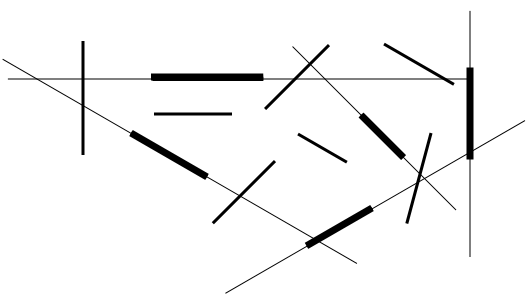
\includegraphics[height=3cm]{rysunki/podzial_h.png}
  \caption{Podział zbioru $F$. Pogrubione elementy należą do zbioru $H$.}
\end{figure} 
Niech $F = \{S_1,\ldots,S_n\}$ będzie zbiorem $n$ rozłącznych odcinków, a $G(F)$ odpowiadającym mu grafem. Zakładamy, że $n$ jest parzyste, w przeciwnym wypadku należy dodać jeden odcinek do zbioru $F$. Pokażemy teraz, że $G(F)$ spełnia twierdzenie Tutte'a \cite{tutte}, a więc posiada skojarzenie doskonałe.
\begin{Definicja}
	Symbolem $o(G)$ oznaczamy liczbę składowych spójności grafu $G$, które posiadają nieparzystą liczbę wierzchołków.
\end{Definicja}
\begin{Twierdzenie} \cite{tutte}
	Spójny graf prosty $G$ o nieparzystej liczbie wierzchołków posiada \emph{doskonałe skojarzenie} wtedy i tylko wtedy, gdy dla każdego $S \subseteq V(G)$ zachodzi $o(G-S) \le |S|$.
\end{Twierdzenie}

\indent Rozważmy dowolny podzbiór $H$ zbioru $F$ oraz niech $S$ będzie zbiorem wierzchołków grafu $G(F)$ reprezentujących elementy $H$. Pokażemy, że liczba składowych spójności grafu $G(F) \setminus S$ wynosi co najwyżej |$S$| = |$H$|.
\\\indent Najpierw usuwamy (z płaszczyzny) wszystkie odcinki, które nie należą do $H$. Następnie, jeden po drugim, przedłużamy elementy $H$ dopóki nie przetną innego elementu $H$, wcześniej przedłużonego odcinka lub nie staną się prostymi bądź półprostymi. Niech $\pi$ oznacza podział płaszczyzny indukowany przez przedłużone elementy zbioru $H$. Zauważmy, że $\pi$ zawiera dokładnie $|H| + 1$ ścian. 
\\\indent Zgodnie z lematem \ref{podgraf indukowany}, liczba składowych spójności grafu $G(F) \setminus S$ jest co najwyżej równa liczbie ścian podziału $\pi$, czyli $|H| + 1$. Można ponadto wykazać, że występują przynajmniej dwie sąsiednie ściany z $\pi$ takie, że odcinki, które je przecinają, należą do tej samej składowej spójności w grafie $G(F) \setminus S$. Stąd wniosek, że liczba elementów zbioru $G(F) \setminus S$ wynosi co najwyżej $|H| = |S|$, co implikuje, że $G(F)$ ma doskonałe skojarzenie $M$. Na tej podstawie możemy stwierdzić, że wystarczy co najwyżej $\ceil{\frac{n}{2}}$ punktów, aby strzec $F$ -- po jednym na każdy wierzchołek krawędzi skojarzenia $M$.
\subsection{Ograniczenie dolne}
\indent Aby uzyskać ograniczenie dolne, należy wskazać $n$-elementowy zbiór $F$, który wymaga $\floor{\frac{2n-3}{5}}$ strażników.
\\\indent Niech $H$ będzie planarnym grafem kubicznym z trójkątną ścianą zewnętrzną, w której wszystkie wierzchołki, poza zewnętrznymi, spełniają założenie, że wektory wychodzące z wierzchołków wzdłuż krawędzi są liniowo niezależne \cite{topp}. Graf $H$ posiada $k$ wierzchołków i $\frac{3k}{2}$ krawędzi.
\\\indent Zamieńmy krawędzie zbioru $H$ na odcinki tak, że na każdy $k - 3$ wewnętrznych wierzchołków przypada trójkątna ściana, w której umieszczamy mały odcinek.

\begin{figure}[ht!]
 \centering
  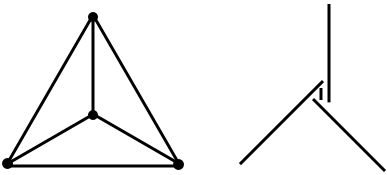
\includegraphics{rysunki/dolna_granica.png}
  \caption{Przekształcenie grafu H.}
  \label{fig:przeksztalcenie h}
\end{figure} 

Odrzucamy trzy krawędzie zewnętrznej ściany $H$, a następnie rozłączamy każdy wierzchołek w jego bliskim sąsiedztwie tak, aby utworzyć zbiór $n = \frac{3k}{2} - 3 + k  - 3$ odcinków (rysunek \ref{fig:przeksztalcenie h}). Żadne dwa z $k - 3$ małych odcinków nie są widoczne z jednego punktu więc $k - 3$ punktów jest potrzebnych, aby strzec taki zbiór. Możemy łatwo sprawdzić, że $k - 3$ punktów jest również wystarczające. Równość $k - 3 = \floor{\frac{2n - 3}{5}}$ kończy dowód twierdzenia \ref{straznicy strzezenie}.

\section{Oświetlanie odcinków}\label{oświetlanie odcinków}
Kolejną wariacją strzeżenia odcinków jest ich oświetlanie. Tym razem, aby strzec odcinek, wymagane jest jego całkowite oświetlenie.
\begin{Definicja}
	Zbiór $S \subseteq \mathbb{R}^2$ źródeł światła \emph{oświetla} zbiór odcinków prostych $F$ wtedy i tylko wtedy, jezeli każdy punkt leżący na odcinku ze zbioru $F$ jest widzialny z co najmniej jednego punktu z $S$.
\end{Definicja} Należy zwrócić uwagę na fakt, że punkt na odcinku może zostać oświetlony przez promień padający na niego z dowolnej strony odcinka.

\begin{Twierdzenie} \cite{illumination}
 Dowolny zbiór $F$ składający się z $n$ rozłącznych odcinków możemy \emph{oświetlić} przy użyciu co najwyżej $\ceil{\frac{2n}{3}} - 3$ źródeł światła
\end{Twierdzenie}

\subsection{Ograniczenie górne}
\indent Niech $F$ = \{$L_1, \ldots, L_n$\} będzie zbiorem $n$ rozłącznych odcinków. Niech $T$ będzie trójkątem, który zawiera wewnątrz wszystkie elementy ze zbioru $F$ oraz niech $F'$ będzie zbiorem zawierającym elementy $F$ oraz trzy odcinki $L_{n+1}$, $L_{n+2}$, $L_{n+3}$ uzyskane przez skrócenie boków trójkąta $T$ o $\epsilon > 0$.
Następnie, niech $H = \{S_1,\ldots,S_n,S_{n+1},S_{n+2},S_{n+3}\}$ będzie rodziną zbiorów złożoną z $n + 3$ ściśle wypukłych oraz wzajemnie wewnętrznie rozłącznych zbiorów (zbiory mogą się stykać tylko w jednym punkcie -- na ich granicach) spełniającą następujące założenia.
\begin{enumerate}
  \item $L_i$ zawiera się w $S_i$, gdzie $i = 1,\ldots,n+3$.
  \item Liczba punktów, w których para elementów rodziny H styka się, jest maksymalna.
\end{enumerate}
\begin{figure}[ht!]
 \centering
  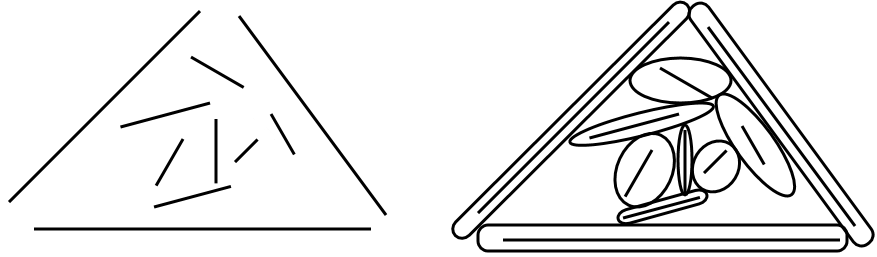
\includegraphics[height=5cm, width=13.5cm]{rysunki/podswietlenie.png}
  \caption{Zbiór $F'$ i rodzina $H$ zbiorów.}
\end{figure} 
Zauważmy, że elementy rodziny $H$ są styczne z przynajmniej trzema innymi elementami z tego zbioru. 
\\\indent Kolejnym krokiem jest stworzenie grafu $G$ poprzez zamianę każdego elementu zbioru $H$ na wierzchołek, przy założeniu, że dwa wierzchołki są sąsiednie, jeżeli odpowiadające im zbiory są styczne.
\begin{figure}[ht!]
 \centering
  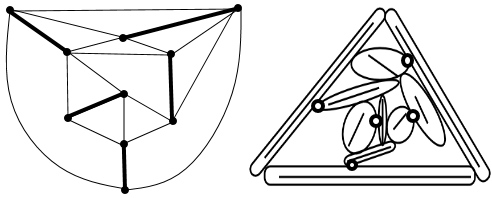
\includegraphics[height=4cm]{rysunki/skojarzenia_zrodla_swiatla.png}
  \caption{Graf G oraz źródła światła}
\end{figure}
Tak stworzony graf jest planarny oraz 2-spójny. Jako że każdy zbiór rodziny $H$ jest styczny z co najmniej trzema innymi zbiorami, stopień każdego wierzchołka grafu $G$ wynosi co najmniej trzy. Zgodnie z twierdzeniem Nishizeki \cite{nishizeki} dla grafu $G$ istnieje skojarzenie $M$ o mocy co najmniej $\ceil{\frac{(n+3)+4}{3}} = \ceil{\frac{n+1}{3}}  + 2$. Dla każdej pary elementów $S_i$ i $S_j$ skojarzonych w $M$ przez krawędź $G$ należy teraz umieścić źródło światła w punkcie ich styczności. W tak wyznaczonym punkcie światło będzie oświetlać odcinki $L_i$ oraz $L_j$ zawierające się, odpowiednio, w $S_i$ oraz $S_j$. Jako że skojarzenie $M$ ma przynajmniej $\ceil{\frac{n+1}{3}} + 2$ elementów, $2(\ceil{\frac{n+1}{3}} + 2)$ elementy ze zbioru $F$ pokryta zostaną przez $\ceil{\frac{n+1}{3}} + 2$ świateł. W każdym z pozostałych elementów, które nie miały skojarzenia, musimy rozmieścić po jednym źródle. W rezultacie uzyskujemy:
$(\ceil{\frac{n+1}{3}} + 2) + ((n + 3) - 2(\ceil{\frac{n+1}{3}})) = n + 5 - \ceil{\frac{n+1}{3}} \le \ceil{\frac{2n}{3}} - 3$.

\subsection{Ograniczenie dolne}
\indent Znana granica dolna nie jest ścisła. Przykładem zbioru, dla którego potrzeba $\floor{\frac{2n-3}{5}}$ źródeł światła, jest np. ten z rysunku \ref{fig:przeksztalcenie h} ze źródłem światła umieszczonym na wewnętrznym odcinku. Z racji dużej różnicy pomiędzy ograniczeniem górnym a dolnym, znalezienie dokładnego wyniku wciąż jest interesującym problemem otwartym. Do tej pory nie udało się znaleźć dowodu chociażby na ograniczenie $\ceil{\frac{n}{2}} + c$, gdzie $c$ jest stałą.

\section{Ukrywanie się za ścianami}
Po raz pierwszy problem ten przedstawili Hurtado, Serra oraz Urrutia \cite{sciany}. Zdefiniowali oni problem w następujący sposób.

\begin{Definicja}\label{ukrywanie definicja}
 Rozpatrzmy zbiór $F$ rozłącznych odcinków . Zbiór $P$ punktów nazywamy \emph{ukrytym} w stosunku do $F$, jeżeli dowolna prosta łącząca dwa punkty ze zbioru $P$ przecina element zbioru $F$.
\end{Definicja}

Dla tak zdefiniowanego problemu, korzystając z twierdzenia Erd{\H o}sa i Szekeresa \cite{erdosszekeres}, uzyskali oni ograniczenie dolne przez $\sqrt{n}$.

\begin{Twierdzenie}\label{moc zbioru ukrytego tw} \cite{illumination}
  Dowolna rodzina $n$ rozłącznych odcinków posiada \emph{zbiór punktów ukrytych} o mocy co najmniej $\sqrt{n}$.
\end{Twierdzenie}

Rozpatrzmy zbiór $F = \{L_1,\ldots,L_n\}$ odcinków takich, że ich rzut na oś OX tworzy rozłączny zbiór. Przez $\alpha_i$ oznaczamy nachylenie odcinka $L_i, i = 1,\ldots,n$ w stosunku do osi OX.
\begin{Lemat}\label{zbior ukryty} \cite{illumination}
  Jeżeli $\alpha_1 < \alpha_2 < \ldots < \alpha_n$, to $F$ posiada ukryty zbiór rozmiaru $n$.
\end{Lemat}

\begin{proof}
	Dla każdego odcinka $L_i$ niech punkt $p_i$ będzie jego środkiem. Wybierzmy punkt $q_i$, poniżej $p_i$, w niewielkiej odległości $\epsilon$ od $L_i, i = 1,\ldots,n$. Rozpatrzmy dwie liczby całkowite $i < j$ oraz odcinek $L_{ij}$ łączący $p_i$ z $p_j$. Jeżeli $\alpha_i$ jest mniejsze niż nachylenie $\alpha_{ij}$ odcinka $L_{ij}$, wtedy wybierając $\epsilon$ wystarczająco małe gwarantujemy, że odcinek łączący $q_i$ z $q_j$ przecina $L_i$. Jeżeli $\alpha_i$ jest większe lub równe $\alpha_{ij}$, to odcinek łączący $q_i$ z $q_j$ przetnie $L_j$. Obrazuje to rysunek \ref{fig:5 zbior ukryty}. A zatem, jeżeli $\epsilon$ jest dostatecznie małe, to  $q_1, \ldots, q_n$ tworzy zbiór ukryty. 
\end{proof}
\begin{figure}[ht!]
  \centering
   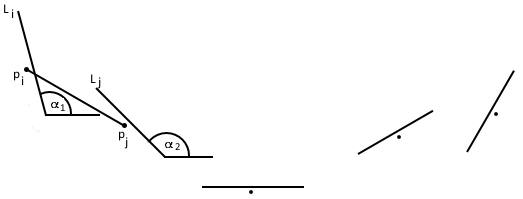
\includegraphics{rysunki/5_odcinkow_zbior_ukryty.png}
   \caption{Zbiór 5 odcinków o rosnącym nachyleniu, który posiada zbiór ukryty o rozmiarze równym 5.}
   \label{fig:5 zbior ukryty}
\end{figure}
\indent Przejdźmy teraz do właściwego dowodu twierdzenia \ref{moc zbioru ukrytego tw}. Rozpatrzmy rodzinę $n$ rozłącznych odcinków. Wybierzmy punkt $p_i$ na każdym z odcinków $L_i$ w taki sposób, aby odcięte $x_1,\ldots, x_n$ punktów dla $p_1,\ldots,p_n$ były różne. Możemy założyć bez straty ogólności, że $x_1$ $<$ $x_2$ $<$ \ldots $<$ $x_n$. Następnie dla każdego $L_i$ wybierzmy odcinek $L'_i$ zawierający się w nim, ze środkiem w punkcie $p_i$, w taki sposób, że rzuty $L'_i,\ldots,L'_n$ na oś OX, tworzą zbiór rozłączny. Rozważmy teraz ciąg nachyleń $L'_1$, \ldots, $L'_n$. Taki ciąg zawiera podciąg rosnący lub malejący o rozmiarze co najmniej $\sqrt{n}$ \cite{illumination}, co biorąc pod uwagę lemat \ref{zbior ukryty}, kończy dowód twierdzenia \ref{moc zbioru ukrytego tw}.

\chapter{K-nadajniki}

\section{Pokrycie płaszczyzny z przeszkodami}\label{sec:knadajniki}
	Ilość sieci wi-fi cały czas rośnie, zarówno w naszych domach jak i w miejscach ogólnodostępnych. Fabila-Monroy oraz Aichholzer \cite{fabilamonroy} zainspirowani postępującą technologią przedstawili nowy problem, ściśle związany z oryginalnym problemem galerii sztuki. Opracowany przez nich wariant, nazywany ,,oświetleniem modemowym'', definiuje strażnika jako bezprzewodowy \emph{nadajnik} o nieskończonym zasięgu oraz możliwości przebicia $k$ ,,ścian''. Ściany są zazwyczaj reprezentowane przez odcinki na płaszczyźnie. Problem zdefiniowali następująco.
\\\indent \emph{Mając dany zbiór przeszkód na płaszczyźnie, liczbę naturalną k $>$ 0 oraz dany obszar, jak wiele nadajników jest czasami potrzebnych a zawsze wystarczających, aby pokryć cały obszar?}  
\\\indent Warto zauważyć, że zagadnienie dla 0-nadajników to klasyczny problem galerii sztuki (strażnicy, którzy nie widzą przez ściany).
\\\indent W wypadku, gdy wymagamy strzeżenia całej płaszczyzny, zakładamy, że nadajnik możemy umieścić wewnątrz ściany, co pozwala nadawać po jej obu stronach.
\subsection{Odcinki prostopadłe}
W tym podrozdziale omówię wariant, w którym przeszkodami będzie zbiór $n$ rozłącznych odcinków prostopadłych, a celem będzie pokrycie całej płaszczyzny. Czyżowicz i inni \cite{czyzowicz} dowiedli, że $\ceil{\frac{n+1}{2}}$ 0-nadajników zawsze wystarcza, a czasami jest koniecznych, aby pokryć całą płaszczyznę, na której znajduje się $n$ rozłącznych prostopadłych odcinków. Ballinger i inni \cite{knadajniki} rozszerzyli to ograniczenie dla \emph{k-nadajników}.

\begin{Twierdzenie} \label{ograniczenie zbiór odcinków prostopadłych} \cite{knadajniki}
  $\ceil{\frac{5n+6}{12}}$ 1-nadajników jest zawsze wystarczających, a $\ceil{\frac{n+1}{4}}$ czasami koniecznych, aby pokryć całą płaszczyznę z $n$ rozłącznymi odcinkami prostopadłymi.
\end{Twierdzenie}
\indent W oparciu o rysunek \ref{fig:ogr_dolne} łatwo wykazać dolną granicę, ponieważ pojedynczy 1-nadajnik może pokryć co najwyżej cztery z $n + 1$ obszarów, z czego wynika, że potrzebujemy $\ceil{\frac{n+1}{4}}$ 1-nadajników dla $n$ prostych równoległych.

\begin{figure}[ht!]
  \centering
  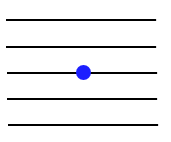
\includegraphics{rysunki/k_nadajniki_ogr_dolne.png}
  \caption{1-nadajnik strzegący czterech obszarów z sześciu}
  \label{fig:ogr_dolne}
\end{figure} 

Ograniczenie górne uzyskamy korzystając z następującego algorytmu:
\begin{itemize}
  \item ze zbioru $S$ wszystkich odcinków usuń odcinki ,,niezależne'';
  \item rozmieść 0-nadajniki;
  \item zwiększ zasięg nadajników o jeden.
\end{itemize}

W pierwszym kroku przedłużamy wszystkie odcinki sekwencyjnie, dopóki się nie przetną lub nie staną się półprostymi, jednocześnie dzieląc płaszczyznę na $n + 1$ ścian. Następnie tworzymy graf widzialności $G(S)$, w którym każdy odcinek ze zbioru $S$ jest wierzchołkiem grafu. Krawędzie między wierzchołkami $s$ i $t$ tworzymy, jeżeli dwa odcinki $s$ i $t$ są słabo widzialne, tzn. istnieją punkty $p$ należący do odcinka $s$ oraz $q$ należący do odcinka $t$ takie, że odcinek $\overline{pq}$ nie przecina żadnego innego odcinka ze zbioru $S$.

\begin{Lemat}\label{0-1-nadajniki} \cite{knadajniki}
  Jeżeli $I$ jest zbiorem niezależnym w grafie $G(S)$, a $T$ jest zbiorem $0$-nadajników, które pokrywają całą płaszczyznę ze zbiorem przeszkód $S \setminus I$, to $T$ jest również zbiorem 1-nadajników, które pokrywają całą płaszczyznę ze zbiorem przeszkód $S$.
\end{Lemat}

\begin{proof}
  Załóżmy, że 0-nadajnik w punkcie $p$ pokrywa punkt $q$ na płaszczyźnie ze zbiorem przeszkód $S \setminus I$. Odcinek $\overline{pq}$ nie może przecinać dwóch lub więcej odcinków ze zbioru $I$, ponieważ wtedy takie odcinki nie byłyby niezależne. Jednocześnie, odcinek $\overline{pq}$ nie przecina żadnego odcinka ze zbioru $S \setminus I$, a więc 1-nadajnik w punkcie $p$ pokrywa $q$ na płaszczyźnie ze zbiorem przeszkód $S$.
\end{proof}

\indent Aby uzyskać możliwie liczny zbiór niezależny w $G(S)$, kolorujemy wierzchołki grafu $G(S)$, a następnie wybieramy najliczniejszą klasę kolorów. Zakładamy, że ściany powstałe przez przedłużenie odcinków w zbiorze $S$ są prostokątne (gdyby były trójkątne, to graf $G(S)$ byłby planarny a więc 4-kolorowalny). 
Tak powstały graf jest 1-planarny oraz 6-kolorowalny \cite{borodin}.

\begin{Definicja}
  Grafem \emph{1-planarnym} nazywamy graf, którego każda z krawędzi może przeciąć inną krawędź co najwyżej raz.
\end{Definicja}
\begin{figure}[ht!]
  \centering
  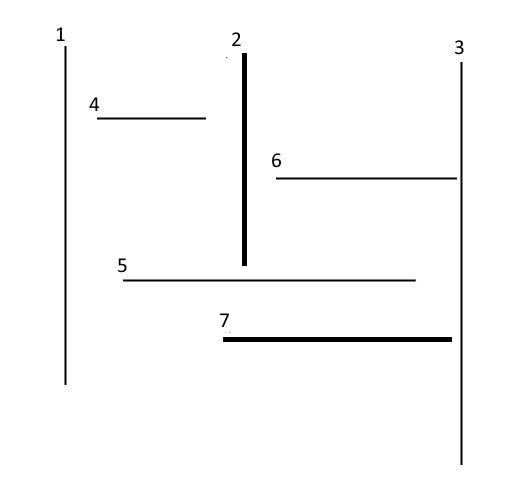
\includegraphics[width=6.5cm]{rysunki/zbior_odcinkow.png}
  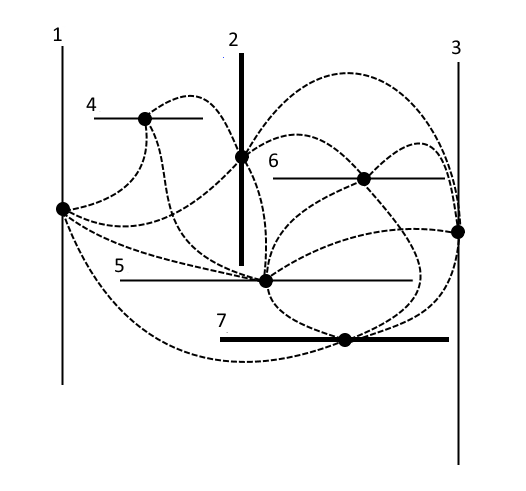
\includegraphics[width=6.5cm]{rysunki/graf_zbioru_odcinkow.png}
  \caption{Zbiór $S$ odcinków oraz graf $G(S)$. Zbiór niezależny został pogrubiony.}
  \label{fig:przedluzone odcinki}
\end{figure} 

\begin{Lemat} \cite{knadajniki}
  Jeżeli $S$ jest zbiorem przedłużonych odcinków prostopadłych, to $G(S)$ jest $1$-planarny.
\end{Lemat}

\indent Aby uzyskać ograniczenie górne, kolorujemy graf $G(S)$ sześcioma kolorami. Najliczniejsza klasa kolorów ma więc nie mniej niż $\frac{n}{6}$ elementów oraz tworzy zbiór niezależny $I$. Pozostały zbiór $S \setminus I$ posiada $\frac{5n}{6}$ odcinków, a więc zgodnie z rezultatem Czyżowicza wystarczy co najwyżej $\ceil{\frac{\frac{5n}{6} + 1}{2}}$ = $\ceil{\frac{5n+6}{12}}$ 0-nadajników, rozmieszczonych na odcinkach zbioru $S \setminus I$. Następnie, zgodnie z lematem \ref{0-1-nadajniki}, zwiększamy moc rozmieszczonych nadajników o jeden, co pozwala strzec całą płaszczyznę ze zbiorem przeszkód $S$.
\begin{figure}[ht!]
  \centering
  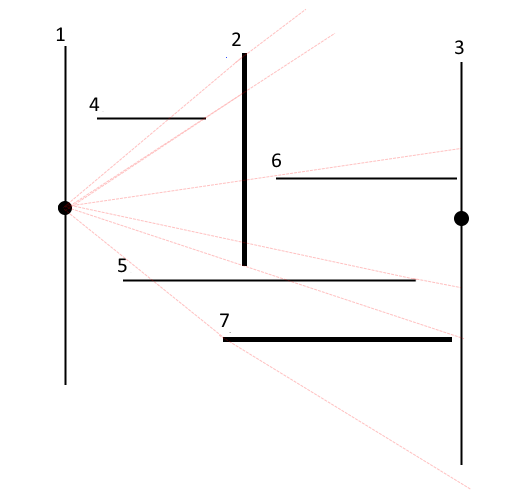
\includegraphics[width=6.5cm]{rysunki/pokrycie_nadajnikami.png}
  \caption{Pokrycie płaszczyzny 1-nadajnikami.}
  \label{fig:pokrycie plaszczyzny}
\end{figure} 

\section{Podział gilotynowy}
Podział gilotynowy $S$ płaszczyzny $\mathbb{R}^2$ otrzymujemy przez dodanie kolejno $s_1,\ldots,s_n$ odcinków prostych w taki sposób, że każdy dodany odcinek $s_i$ dzieli dowolną ścianę podzbioru $S_{i-1}$ na dwie nowe ściany tworząc nowy podział $S_i$. Za ścianę $S_0$ przyjmujemy całą płaszczyznę. Zauważmy, że ściany podziału gilotynowego są wypukłe.

\begin{Lemat}\label{sasiednie sciany strzega F} \cite{knadajniki}
  Niech $F$ będzie ścianą podziału gilotynowego $S$. Jeżeli każda inna ściana, która współdzieli krawędź ze ścianą $F$, posiada wewnątrz 1-nadajnik, to taki zbiór nadajników pokrywa całą ścianę $F$.
\end{Lemat}
\begin{proof}
\indent Rozpatrzmy odcinek $s_i$, którego dodanie tworzy ścianę $F$. Przed dodaniem odcinka $s_i$ podział $S_{i-1}$ zawierał jedną ścianę, która została podzielona na dwie części $F$ oraz $F'$ przez $s_i$. 
% \begin{figure}[ht!]
%    \centering
%    \label{podzial F przez s_i}
%    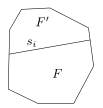
\includegraphics[width=9cm,height=6cm]{rysunki/podzial_F.png}
%    \caption{Ściana $F$ oraz $F'$ po dodaniu odcinka $s_i$.}
% \end{figure} 

W dalszym procesie ściana $F$ nie będzie już dzielona, ale możemy podzielić ścianę $F'$ uzyskujac kolejne ściany $F'_1, \ldots, F'_k$, takie, że $F'_j \subseteq F'$ oraz $F'_j$ dzieli część odcinka $s_i$ ze ścianą $F$ dla każdego $j \in \{1,\ldots,k\}$ (rysunek \ref{fig:podzial F' na kolejne ściany}).

\begin{figure}[ht!]
  \centering
  \includegraphics[width=9cm,height=6cm]{rysunki/podzial_F'.png}
  \caption{Kolejne podziały ściany $F'$.}
  \label{fig:podzial F' na kolejne ściany}
\end{figure} 
Tymczasowo usuńmy odcinek $s_i$. W ten sposób uzyskalismy podział $S'$, przedłużając odcinki, którymi wcześniej dokonaliśmy podziału ściany $F'$ (rysunek \ref{fig:podzial po usunieciu si}).

\begin{figure}[ht!]
  \centering
  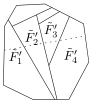
\includegraphics[width=9cm,height=6cm]{rysunki/usuniete_si.png}
  \caption{Podział płaszczyzny po usunięciu odcinka $s_i$.}
  \label{fig:podzial po usunieciu si}
\end{figure} 

Po tej operacji każda ze ścian $F'_j$ w $F$ powiększa się w $S'$, a dodatkowe części ścian sumują się do $F$. Widzimy, że każdy z $1$-nadajników rozmieszczonych wewnątrz ścian $F_j$ pokrywa przynajmniej obszar ściany $F'_j$, a więc razem nadajniki w $F_1,\ldots,F_k$ pokryją ścianę $F$ (rysunek \ref{fig:pokrycie f}).
\end{proof}

\begin{figure}[ht!]
  \centering
  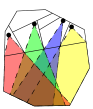
\includegraphics[width=9cm,height=6cm]{rysunki/pokrycie_f.png}
  \caption{Nadajniki każdej ze ścian strzegące całą ścianę $F$.}
  \label{fig:pokrycie f}
\end{figure} 

\begin{Twierdzenie} \cite{knadajniki}
  Dowolny podział gilotynowy możemy strzec przez co najwyżej $\floor{\frac{n+1}{2}}$ $1$-nadajników.
\end{Twierdzenie}
\begin{proof}
	Rozpatrzmy graf dualny $T$ podziału. $T$ jest triangulacją o $n + 1$ krawędziach. Niech $M$ będzie maksymalnym skojarzeniem w grafie $T$. Każdy nieskojarzony wierzchołek jest sąsiedni tylko do wierzchołków skojarzonych (w przeciwnym przypadku skojarzenie nie byłoby maksymalne). Niech $G$ będzie zbiorem 1-nadajników uzyskanych przez rozmieszczenie ich na krawędziach podziału odpowiadającym krawędziom z $M$. W takim wypadku |$G$| = |$M$| $\le \floor{\frac{n+1}{2}}$. Dla każdej ściany $F$ z $S$, $F$ albo zawiera 1-nadajnik w $G$ albo wszystkie sąsiednie ściany, które dzielą krawędź z $F$, zawierają 1-nadajnik w $G$. W pierwszym przypadku $F$ jest oczywiście strzeżona. Natomiast w drugim przypadku, zgodnie z lematem \ref{sasiednie sciany strzega F}, ściana $F$ również jest strzeżona. Dlatego $G$ jest zbiorem 1-nadajników, które strzegą wszystkie ściany $F$ o mocy co najwyżej $\floor{\frac{n+1}{2}}$.
\end{proof}

\chapter{Strażnicy na siatkach}
\section{Siatki 2D} \label{sec:siatki}
W 1986 roku Simeon Ntafos przedstawił koncept strażników strzegących specjalnej klasy wielokątów -- siatek \cite{ntafos}.
Przez \emph{siatkę} $P$ rozumiemy spójny zbiór punktów należących do poziomych oraz pionowych odcinków prostych (rysunek \ref{fig:siatka 2d}). Możemy na nią spojrzeć jak na wielokąt prostokątny z dziurami, który składa się z bardzo cienkich korytarzy.
Strażnik będący w punkcie $x$ siatki $P$ \emph{widzi} punkt $y$ siatki $P$ jeżeli odcinek $xy$ należy do siatki $P$ (czyli zawiera się w korytarzu siatki).
 \begin{figure}[ht!]
   \centering
   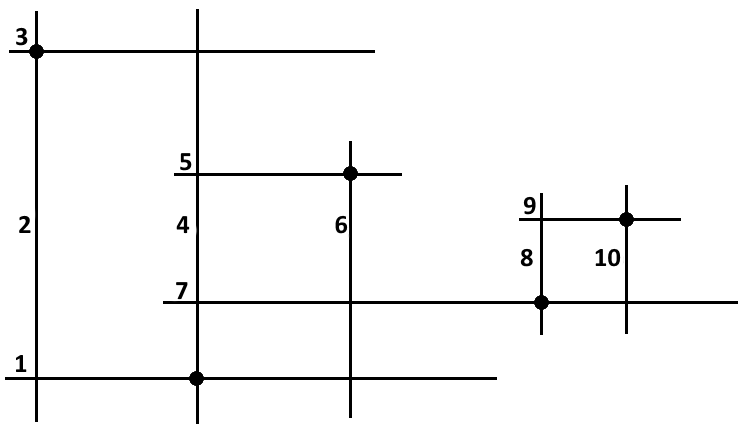
\includegraphics[width=14cm,height=6cm]{rysunki/przykladowa_siatka.png}
   \caption{Siatka strzeżona przez pięciu strażników.}
   \label{fig:siatka 2d}
 \end{figure} 

\begin{Twierdzenie} \cite{ntafos}
	Minimalna liczba strażników potrzebna, aby \emph{strzec siatkę} o $n$ odcinkach wynosi $n - m$, gdzie $m$ to moc najliczniejszego skojarzenia w grafie przecięć, które można znaleźć w czasie $\theta(n^{2.5})$
\end{Twierdzenie}

Ntafos zaproponował elegancki algorytm, aby znaleźć minimalną liczbę strażników potrzebną do strzeżenia siatki.

\begin{proof}
Aby strzec całej siatki, przynajmniej jeden strażnik musi znajdować się w każdym korytarzu. Niech $G$ będzie grafem przecięć siatki, w którym każdy wierzchołek z grafu $G$ odpowiada odcinkowi, a dwa wierzchołki są połączone krawędzią wtedy i tylko wtedy, gdy odpowiadające im odcinki przecinają się.

 \begin{figure}[ht!]
   \centering
   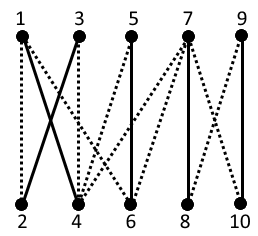
\includegraphics{rysunki/graf_skojarzen.png}
   \caption{Graf przecięć siatki. Skojarzenie oznaczono linią ciągłą.}
   \label{fig:graf przeciec}
 \end{figure} 

 Najliczniejsze skojarzenie dla dowolnego grafu $G = (V,E)$ można znaleźć w czasie O($|V|^{2.5}$) \cite{even}. Jako że graf $G$ jest dwudzielny, ponieważ przecięcia występują tylko pomiędzy korytarzamia pionowymi i poziomymi, problem znalezienia najliczniejszego skojarzenia sprowadza się do problemu kojarzenia małżeństw, który da się rozwiązać w czasie $O(|V|^{1/2}|E|)$, gdzie $V$ to zbiór wierzchołków a $E$ to zbiór krawędzi w grafie dwudzielnym \cite{even}. Dla siatki o $n$ odcinkach $|V| = n$, a maksymalna ilość krawędzi to $|E| = O(n^2)$, więc w najgorszym przypadku najliczniejsze skojarzenie znajdziemy w czasie $O(n^{2.5})$.
 \\\indent Aby strzec siatkę w całości, każdy odcinek wymaga strażnika, a więc rozmieszczenie ich na przecięciach korytarzy pozwala strzec co najwyżej dwa odcinki. Stąd uzyskujemy minimalną liczbę strażników wynoszącą $\ceil{\frac{n}{2}}$ dla siatki o $n$ odcinkach. Jeżeli graf posiada skojarzenie doskonałe o rozmiarze $\ceil{\frac{n}{2}}$, wtedy taka sama ilość strażników jest wystarczająca. Należy ich rozmieścić w każdym przecięciu korytarzy odpowiadającemu skojarzeniu w grafie. Jeżeli najliczniejsze skojarzenie ma moc $m$, wtedy rozmieszczenie w odpowiadających im przecięciach strzeże $2m$ odcinków. W każdym z pozostałych $n - 2m$ odcinków musi zostać umieszczony jeden strażnik, co w sumie daje nam $m + n - 2m = n - m$ strażników. Jest to jednocześnie dolne ograniczenie: jeżeli mniej niż $n - m$ strażników wystarcza, wtedy więcej niż $m$ strażników musi kryć dwa odcinki, a to daje nam skojarzenie o rozmiarze większym niż $m$, co nie jest możliwe.
\end{proof}

 \section{Siatki 3D}
 	Ntafos przedstawił również zagadnienie strzeżenia siatki w trzech wymiarach, które należy do klasy problemów NP-zupełnych \cite{ntafos}. Dowód opiera się na redukcji do problemu pokrycia wierzchołkowego grafu, stopnia co najwyżej trzy, który to problem należy do klasy problemów NP-zupełnych \cite{garey}.
\begin{Definicja}
	\emph{Pokryciem wierzchołkowym} grafu $G = (V,E)$ nazywamy podzbiór $V_0 \subseteq V$ takich wierzchołków grafu, że każda krawędź z $G$ jest incydentna z przynajmniej jednym wierzchołkiem z $V_0$.
\end{Definicja}
Naszym celem jest stworzenie trójwymiarowej siatki $P$, którą możemy pokryć co najwyżej $g(K)$ strażnikami wtedy i tylko wtedy, gdy istnieje pokrycie wierzchołkowe $G$ o mocy co najwyżej $K$.
W tym celu etykietujemy wszystkie wierzchołki grafu $G = (V,E)$ kolejnymi liczbami $1,2,\ldots,n = |V|$. Następnie, przypisujemy wierzchołki punktom siatki wzdłuż prostej poprowadzonej przez punkty $(0,0,0)$ i $(1,1,1)$ tak, aby każdy wierzchołek $i$ otrzymał punkt siatki $v_i = (3i, 3i, 3i)$. Krawędzie $G$ reprezentowane są przez odcinki łączące węzły siatki. Jako że każdy wierzchołek grafu $G$ jest stopnia co najwyżej trzy, każdej incydentnej krawędzi możemy przypisać jeden z kierunków $(x,y,z)$.
\\\indent Załóżmy teraz, że wszystkie krawędzie incydentne z wierzchołkami $1,\ldots,i - 1$ grafu $G$ zostały przypisane do ścieżek siatki $P$ oraz rozpatrzmy krawędź ${i,j}, i < j$. Przyjmujemy, że ścieżka z $v_i$ do $v_j$, dla $i < j$, wychodzi z $v_i$ dodatnią osią $+x$, $+y$ lub $+z$, a wchodzi do $v_j$ ujemną osią $-x$, $-y$ lub $-z$. Skoro stopień wierzchołka $i$ wynosi co najwyżej trzy, jedna z trzech osi $+x$, $+y$ lub $+z$ rozpoczynająca się w $(3i, 3i, 3i)$ nie zawiera ścieżki dotychczas skonstruowanej siatki $P$. Załóżmy, że oś $+x$ jest wolna. W takim wypadku łączymy $v_i = (3i, 3i, 3i)$ z $v_j = (3j, 3j, 3j)$ trzema odcinkami:
\begin{itemize}
	\item $(3i, 3i, 3i) \rightarrow (3j, 3i, 3i)$;
	\item $(3j, 3i, 3i) \rightarrow (3j, 3j, 3i)$;
	\item $(3j, 3j, 3i) \rightarrow (3j, 3j, 3j)$.
\end{itemize}
Oczywiście, powyższe odcinki nie mogą przecinać się z żadnymi już istniejącymi ścieżkami. Przykład takiego połączenia widać na rysunku \ref{fig:nowe sciezki} w przypadku, gdy wolna jest oś $+x$, $+y$ lub $+z$.
\begin{figure}[ht!]
  \centering
  a)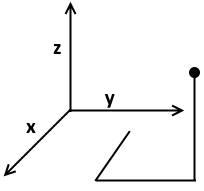
\includegraphics[width=4cm,height=5cm]{rysunki/wolne_x.png}
  b)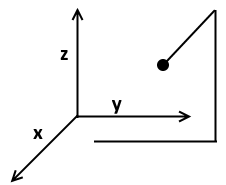
\includegraphics[width=4cm,height=5cm]{rysunki/wolne_y.png}
  c)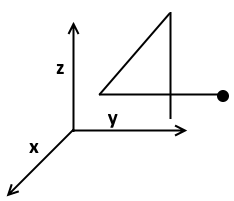
\includegraphics[width=4cm,height=5cm]{rysunki/wolne_z.png}
  \caption{Nowo powstałe ścieżki w przypadku wolnych osi $+x$, $+y$ lub $+z$.}
  \label{fig:nowe sciezki}
\end{figure} 
\\\indent Zajmiemy się teraz przypadkiem, w którym fragment ścieżki pomiędzy węzłami $v_i$ i $v_j$ nakłada się ze ścieżką łącząca $v_k$ z $v_j$ wzdłuż osi $-z$, dla $k < i < j$. W takiej sytuacji przynajmniej jedna z osi $-x$ lub $-y$ musi być wolna. Jeżeli jest to oś $-x$, zmieniamy ścieżkę zgodnie z rysunkiem \ref{fig:nakladanie}(a), jeżeli $-y$, to wtedy musimy poprawić ścieżkę zgodnie z rysunkiem \ref{fig:nakladanie}(b). Analogicznych operacji dokonamy jeżeli zajęta będzie oś $-x$ i $-y$.

\begin{figure}[ht!]
  \centering
  a)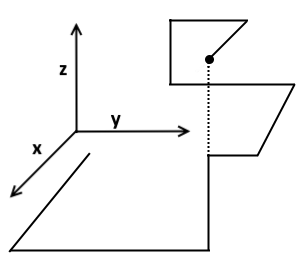
\includegraphics[width=6cm,height=5cm]{rysunki/zajete_z.png}
  b)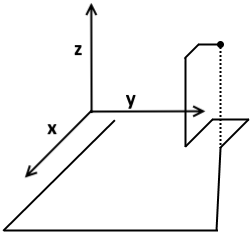
\includegraphics[width=6cm,height=5cm]{rysunki/zajete_z2.png}
  \caption{Omijanie zajętej ścieżki w przypadku wolnej osi $-x$ oraz $-y$}
  \label{fig:nakladanie}
\end{figure} 

Tak powstała krawędź składa się z dziewięciu odcinków. W przypadku, gdy zajdzie potrzeba ominięcia jeszcze jednej krawędzi uzyskamy ścieżkę składającą się z 15 odcinków \cite{orourke}.
\\\indent Po stworzeniu siatki wg powyższego opisu uzyskamy w sumie $e = e_3 + e_9 + e_{15}$ krawędzi grafu $G$, gdzie, odpowiednio, $e_3$  jest liczbą krawędzi, którym odpowiadają ścieżki złożone z 3 odcinków, $e_9$ -- z 9 odcinków oraz $e_{15}$ -- z 15 odcinków.

\begin{Lemat} \cite{orourke}
	Pokrycie wierzchołkowe grafu $G$ o rozmiarze $K$ istnieje wtedy i tylko wtedy, gdy istnieje pokrycie siatki $P$ powstałej wg powyższej konstrukcji przez $g = K + e_3 + 4e_9 + 7e_{15}$ strażników.
\end{Lemat}

\begin{proof} 
	Załóżmy, że istnieje pokrycie wierzchołkowe $C$ grafu $G$ o rozmiarze $K$. Następnie, rozmieśćmy strażnika w każdym przecięciu siatki $P$, które odpowiada wierzchołkowi w $C$.
	Niech $p_3$ będzie ścieżką złożoną z 3 odcinków w $P$ pomiędzy $v_i$ a $v_j$. Ponieważ $C$ jest pokryciem wierzchołkowym, przynajmniej w jednym z węzłów $v_i$ lub $v_j$ znajduje się strażnik, a więc potrzebujemy jeszcze jednego strażnika, aby strzec całą $p_3$. Podobna sytuacja występuje dla 1-elementowej ścieżki $p_9$ pomiędzy $v_i$ oraz $v_j$. Jeden z węzłów $v_i$ lub $v_j$ jest już strzeżony więc dodatkowo potrzebujemy 4 strażników. Dla 15-elementowej ścieżki $p_{15}$ potrzebujemy 7 dodatkowych strażników, co w rezultacie daje nam $K + e_3 + 4e_9 + 7e_{15}$ strażników.

	\indent Załóżmy teraz, że aby strzec siatkę $P$ wystarczy $K + e_3 + 4e_9 + 7e_{15}$ strażników. Każda z 3-elementowych ścieżek wymaga jednego strażnika w wewnętrznym rogu. Ścieżka złożona z dziewięciu odcinków wymaga czterech strażników rozmieszczonych w wewnętrznych rogach, a 15-odcinkowa -- siedmiu. Stąd uzyskujemy sumę $e_3$ + 4$e_9$ + 7$e_{15}$ strażników rozmieszczonych w miejscach innych niż punkty siatki, którym odpowiadają wierzchołki grafu $G$. Pozostało nam jeszcze $K$ strażników, których możemy umieścić tylko w punktach siatki odpowiadających wierzchołkom grafu $G$. Załóżmy więc, że strażnicy rozmieszczeni w tych punktach nie tworzą pokrycia wierzchołkowego grafu $G$. W takim wypadku krawędź ${i, j}$ z $G$ nie jest incydentna z żadnym wierzchołkiem należącym do pokrycia wierzchołkowego, a więc odpowiadająca jej ścieżka w siatce $P$ nie posiada strażników zarówno w $v_i$ ani w $v_j$. Wiemy jednak, że aby pokryć np. ścieżkę 3-elementową, jeden strażnik w wewnętrznym ,,rogu'' jest w stanie strzec tylko dwa z trzech odcinków. Analogiczna sytuacja występuje dla ścieżek złożonych z dziewięciu oraz piętnastu odcinków, w których, odpowiednio, czterech i siedmiu strażników jest w stanie strzec co najwyżej osiem i czternaście z dziewięciu oraz piętnastu odcinków. Stąd wnioskujemy, że jeżeli owych pozostałych, $K$ strażników nie stanowi pokrycia wierzchołkowego, to nie możemy pokryć siatki $P$ przez $K + e_3 + 4e_9 + 7e_{15}$ strażników. 
\end{proof}

\begin{Twierdzenie} \cite{ntafos}
	Zagadnienie strzeżenia trójwymiarowej siatki przez minimalną liczbę strażników należy do klasy problemów NP-zupełnych.
\end{Twierdzenie}
\begin{proof} 
	Ponieważ strażnicy mogą być rozmieszczeni tylko na skrzyżowaniach siatki lub w jej rogach, których jest skończona (wielomianowa) liczba, rozwiązanie możemy zgadnąć oraz sprawdzić w czasie wielomianowym. Problem pokrycia wierzchołkowego należy do klasy problemów NP-zupełnych a więc zagadnienie zredukowanie do tego problemu również należy do klasy problemów NP-zupełnych.
\end{proof}

\chapter{Problem pościgu i ucieczki w grafie}
\section{Gra w złodzieja i policjanta}\label{sec:poscig}
Mając dany graf $G$, zbiór reguł $S$, liczbę całkowitą $k$, oraz dwa warunki $T_1$ i $T_2$, gra zaczyna się od rozmieszczenia przez gracza pierwszego (policjanta, oznaczenie $A$) nie więcej niż $k$ żetonów na wierzchołkach grafu $G$. Gracz numer dwa (złodziej, oznaczenie $Z$) rozmieszcza jeden żeton na dowolnym wierzchołku $G$. Następnie gracze przesuwają swoje żetony, zgodnie z regułami ze zbioru $S$, dopóki nie zajdzie jeden z warunków $T_i$. Jeżeli końcowa konfiguracja spełnia warunek $T_1$ -- wygrywa gracz $A$ (policjant), w przeciwnym wypadku wygrywa gracz $Z$ (złodziej). W klasycznej wersji gry obaj gracze znają rozmieszczenie wszystkich żetonów, a jedynym warunkiem końcowym jest, aby żeton gracza $A$ oraz $Z$ znajdował się na tym samym wierzchołku grafu $G$.
Reguły $S$ wyglądają następująco.
\begin{enumerate}
  \item Gracze wykonują ruchy na przemian
  \item Gracz $A$ w swojej kolejce może odmówić ruchu lub przesunąć wzdłuż krawędzi jeden ze swoich żetonów na wierzchołek sąsiedni z aktualnie zajmowanym.
  \item Gracz $Z$ w swojej kolejce może odmówić ruchu lub przesunąć wzdłuż krawędzi swój żeton na wolny wierzchołek sąsiedni z wierzchołkiem aktualnie zajmowanym.
\end{enumerate}

Problem ma praktyczne zastosowanie na przykład w planowaniu ruchu robotów, kiedy ważnym jest, aby nie następowały kolizje lub poważniejsze zderzenia.

Zagadnienie pościgu i ucieczki w kracie, opiera się na przeszukiwaniu jej w taki sposób, aby po wykonaniu $n$ kroków policjant zauważył złodzieja (tzn. znajdował się w tym samym wierszu lub w tej samej kolumnie) lub, w trudniejszym wariancie, znajdował się w tym samym wierzchołku co złodziej. Taką sytuację uznajemy za zwycięstwo goniącego, w przeciwnym wypadku zwycięża złodziej. Obaj uczestnicy poruszają się tylko po wierszach i kolumnach siatki z ograniczoną prędkością.

Najprostszym przykładem gry w postaci ogólnej, w której zawsze zwycięża policjant, jest drzewo oraz współczynnik $k = 1$. W takim przypadku policjant w każdym kolejnym ruchu zbliża się do drugiego gracza, który w żadnym momencie nie jest w stanie go minąć, co zawsze prowadzi do zwycięstwa goniącego.

\subsection{Wariant Sugiharu i Suzuki}
W tym rozdziale zajmę się wariantem gry przedstawionym przez Sugiharu i Suzuki \cite{sugiharu}, w którym warunkiem zwycięstwa policjanta jest zauważenie złodzieja, a gra odbywa się na grafie $G$ przypominającym prostokątną kratę.
Przez kratę rozumiemy graf $G_{n,m}$, gdzie $n$ to liczba wierzchołków, a $m$ liczba krawędzi, z których każda ma długość jeden. Zakładamy również, że graf jest rozpięty na płaszczyźnie z punktem poczatkowym $v_{0,0}$ w lewym górnym wierzchołku.
\begin{figure}[ht!]
   \centering
    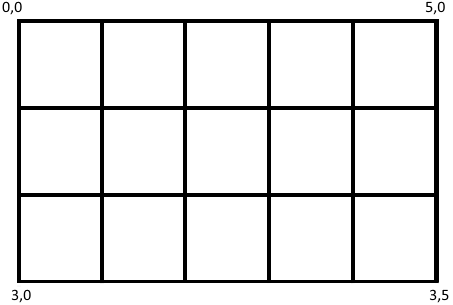
\includegraphics[height=5cm]{rysunki/siatka_3_5.png}
    \caption{Krata $G_{3,5}$.}
\end{figure}

\begin{Definicja}
  Gracz $A$ \emph{jest widoczny} dla gracza $Z$ wtedy i tylko wtedy, gdy obaj znajdują się w tej samej kolumnie lub w tym samym wierszu kraty, niezależnie od odległości która ich dzieli.
\end{Definicja}

Gracz przesuwają swoje żetony tylko po krawędziach grafu, a szybkość ruchu jest określona przed rozpoczęciem gry.
W tym wariancie gry gracze nie mają całkowitej wiedzy o pozycjach, które zajmują. Tylko złodziej posiada wszystkie informacje o miejscach, które zajmuje policjant. Ścigający za to nie wie nic o pozycji uciekającego, dopóki nie zostanie on zauważony. Dodatkowo, ruchy gracza $A$ są z góry określone, zanim gra w ogóle się rozpocznie.
Zasady $S$ wyglądają następująco.
\begin{enumerate}
  \item Gracze poruszają się w czasie rzeczywistym.
  \item Prędkość ścigającego jest stała i wynosi $S_n$.
  \item Uciekający porusza się z prędkością co najwyżej $S_c$.
\end{enumerate}

\noindent Warunki kończące grę są następujące.
\begin{enumerate}
  \item Złodziej został zauważony przez policjanta.
  \item Uciekający zawsze jest w stanie zapobiec zwycięstwu policjanta.
\end{enumerate}

Podobnie jak zwykły problem gonitwy i ucieczki, również ta odmiana jest całkowicie deterministyczna i zależy od parametrów początkowych gry. Naszym celem jest określenie warunków, w których zawsze zwycięża gracz pierwszy. 

\begin{Twierdzenie} \cite{poscig}
	Jeżeli $S_c \le n + 1$, policjant zawsze wygrywa dla stałej $S_n = n + 1$.
\end{Twierdzenie}
\begin{proof}
	Aby dowieść powyższego twierdzenia, skorzystamy z następującego algorytmu.
	\begin{enumerate}
		\item Gracz pierwszy porusza się w dół kolumną $k$, startując w wierzchołku $(0,k)$, przechodząc przez wierzchołek $(n, k)$ a kończąc ruch w $(n, k + 1)$. Pokonanie takiej trasy zajmuje jedną jednostkę czasu.
		\item Następnie, przesuwa się w górę kolumną $k + 1$, kończąc ruch w wierzchołku $(0,k)$. Pokonanie takiej ścieżki również zajmuje jedną jednostkę czasu.
		\item Powtarzamy ruch nr 1.
		\item Wykonuje ruch w górę kolumną $k + 1$, kończąc go w wierzchołku $(0,k + 1)$, tracąc $\frac{n}{n+1}$ jednostki czasu.
	\end{enumerate}
	\begin{figure}[ht!]
	  \centering
	  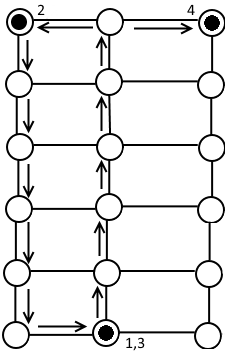
\includegraphics[height=6cm]{rysunki/schemat_ruchu.png}
	  \caption{Trasa pokonana przez gracza pierwszego w wyniku algorytmu.}
	\end{figure} 

	Czas $t_{k+1}$, którego potrzebował gracz pierwszy, aby wykonać powyższy schemat wynosi $t_{k+1} = t_k + 3 + \frac{n}{n+1}$.
	Załóżmy, że po wykonaniu powyższych ruchów gracz $Z$ albo został już zauważony, co kończy grę, lub znajduje się w części siatki ograniczonej przez wierzchołki $[(0,k + 1), (n, n)]$.
	\\\indent Jako że gra toczy się dalej, gracz $Z$ nie może znajdować się w pierwszym wierszu ani $k-tej$ kolumnie, ponieważ wtedy byłby widoczny dla policjanta. W czasie $t_k$ gracz $Z$ znajduje się w części kraty ograniczonej przez wierzchołki $[(0,k + 1), (n, n)]$ i próbuje się przedostać do części $[(0,0), (n, k + 1)]$ (rysunek \ref{fig:miejsceucieczki}).

	\begin{figure}[ht!]
	  \centering
	  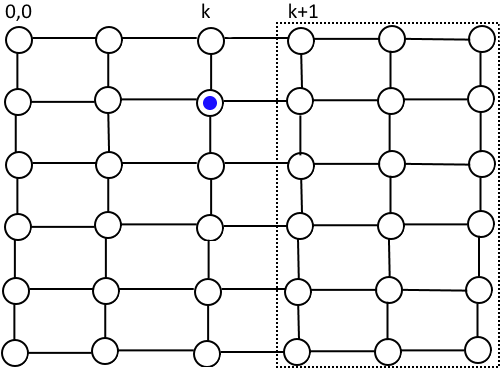
\includegraphics[height=5cm]{rysunki/podsiatka.png}
	  \caption{Złodziej znajduje się w części kraty zaznaczonej linią przerywaną}
    \label{fig:miejsceucieczki}
	\end{figure} 

	\indent W czasie, kiedy policjant przemieszcza się kolumną $k$, złodziej może zbliżać się do niej wierszem $j$. Policjant dotrze do wierzchołka $(j,k)$ po czasie $\frac{j}{n+1}$ a więc do tego momentu złodziej musi znajdować się powyżej (lub poniżej) wiersza $j$. Wynika z tego, że w momencie kiedy gracz $A$ kończy pierwszy ruch, gracz $Z$ znajduje się w odległości $\frac{1-j}{n+1} - \epsilon$ pomiędzy wierzchołkiem $(j,k + 1)$ a wierzchołkiem $(j,k)$. Obrazuje to rysunek \ref{fig:pierwszy krok}.
	\begin{figure}[ht!]
	  \centering
	  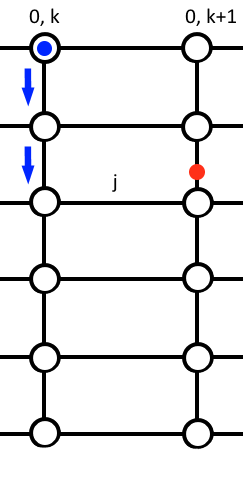
\includegraphics[width=5cm,height=7cm]{rysunki/poscig_1.png}
	  \caption{Pierwszy etap pościgu.}
	  \label{fig:pierwszy krok}
	\end{figure}
	\\\indent Gracz $A$ ponownie przekroczy wiersz $j$ w drugim kroku algorytmu po upływie $\frac{n-1}{n+1}$ czasu. Do tego momentu gracz $Z$ musi przejść cały wiersz i znaleźć się w kolumnie $k$. Żeby tego dokonać musi przemieścić się o $\frac{j}{n+1}$ + $\delta$ w ciągu $\frac{n-1}{n+1}$ jednostek czasu. Daje nam to ograniczenie $j < \frac{n}{2}$.
	\\\indent Pomiędzy momentem, kiedy policjant przekracza wiersz $j$ w kroku drugim a przejściem do wierzchołka $(0,k)$ mija $\frac{j}{n+1}$ jednostki czasu. W sumie mijają dwie jednostki czasu od momentu $t_k$. Złodziej startując w kolumnie $j + 1$ i poruszając się wzdłuż wiersza $j$ nie ma wystarczajaco dużo czasu aby przesunąć się do wiersza $j - 1$ lub $j + 1$ ponieważ nie może rozpocząć ruchu dopóki pierwszy gracz nie przekroczy wiersza $j$. Więc w momencie, kiedy ścigający kończy ruch nr 2, gracz $Z$ musi znajdować się w odległości nie większej niż $\frac{j}{n+1} - \gamma$ od $(k,j)$. 

	Widać to na poniższym rysunku. 
	\begin{figure}[ht!]
	  \centering
	  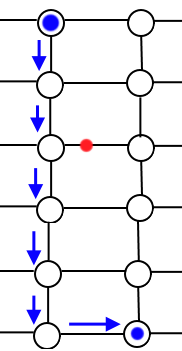
\includegraphics[width=5cm,height=7cm]{rysunki/poscig_2.png}
    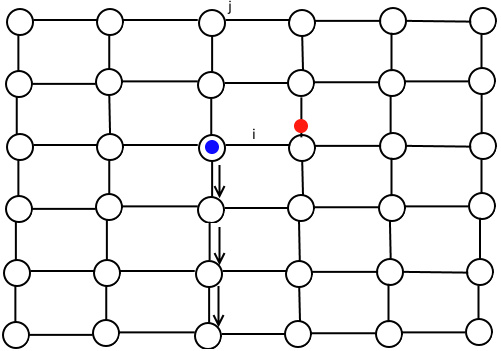
\includegraphics[width=5cm,height=7cm]{rysunki/poscig_3.png}
	  \caption{Drugi etap pościgu}
	  \label{fig:drugi krok}
	\end{figure}

	\indent Gracz $A$ osiąga $(j,k)$ w kroku trzecim po upływie kolejnych $\frac{j}{n+1}$ jednostek. W tym samym czasie gracz $Z$ nie jest w stanie osiągnąć kolumny $k - 1$ ani wrócić do $k + 1$ a więc zostaje zauważony.
	\begin{figure}[ht!]
	  \centering
	  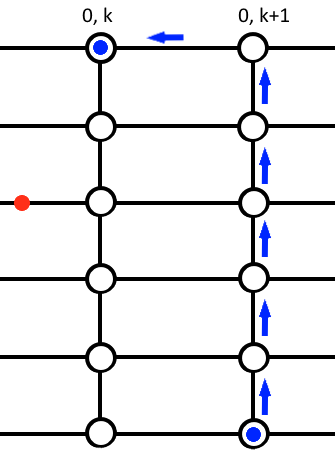
\includegraphics[width=5cm,height=7cm]{rysunki/poscig_4.png}
	  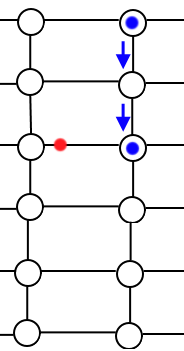
\includegraphics[width=5cm,height=7cm]{rysunki/poscig_5.png}
	  \caption{Ostatni etap pościgu.}
	  \label{fig:ostatni etap poscigu}
    \vspace{5in}
	\end{figure} 

	\indent Ponieważ policjant widzi przez całą długość wiersza/kolumny, takie samo rozumowanie będzie miało zastosowanie jeżeli złodziej będzie rozpoczynał swój ruch z każdej kolumny $k > j + 1$. W ten sposób jeżeli gracz A rozpocznie grę w punkcie $(0,0)$ oraz wszystkie założenia początkowe będą spełnione zawsze zakończy grę sukcesem w czasie nie większym niż $t_n < n$.
\end{proof} 
\summary
Avis i Toussaint \cite{avis} korzystając z metody przedstawionej przez Fiska \cite{fisk}, opisanej w rozdziale \ref{sec:klasyczny}, uzyskali algorytm który w czasie $0(n logn)$ jest w stanie znaleźć rozwiązanie klasycznego problemu galerii sztuki dla wielokątów prostych. Opisany w dalszej części rozdziału problemu dla wielokątów z dziurami wymaga co najwyżej $\floor{\frac{n+2h}{3}}$ = $\ceil{\frac{t}{3}}$ strażników.

W rozdziale \ref{sec:strzezenie odcinkow} opisuję zagadnienie strzeżenia zbioru odcinków rozłącznych.
Aby strzec dowolny zbiór $n$ rozłącznych odcinków prostych zawsze wystarcza $\ceil{\frac{n}{2}}$ a czasami potrzeba $\floor{\frac{2n-3}{5}}$ strażników. W dalszej części rozdziału omawiam inny wariant strzeżenia zbioru - oświetlanie. Aby oświetlić dowolny zbiór odcinków potrzebujemy nie więcej niż $\ceil{\frac{2n}{3}} - 3$ źrodeł światła. Ograniczenie dolne jest wciąż problemem otwartym. Na koniec zajmuje się problemem znajdowania zbioru ukrytego, który dla dowolnej rodziny $n$ rozłącznych odcinków posiada moc co najmniej $\sqrt{n}$

Kolejny rozdział opisuje $K$-nadajniki \ref{sec:knadajniki} a dokładnie pokrycie płaszczyzny z przeszkodami oraz podział gilotynowy. Aby pokryć płaszczyznę z $n$ rozłącznymi odcinkami prostopadłymi zawsze wystarcza $\ceil{\frac{5n+6}{12}}$ $1$-nadajników a $\ceil{\frac{n+1}{4}}$ jest czasami koniecznych. Natomiast dowolny podział gilotynowy można strzec przez co najwyżej $\floor{\frac{n+1}{2}} 1$-nadajników.

Następnym omówionym zagadnieniem są strażnicy na siatkach \ref{sec:siatki}. Aby strzec siatkę w dwóch wymiarach potrzebnych jest co najmniej $n - m$ strażników, gdzie $m$ to moc najliczniejszego skojarzenia grafu przecięć siatki. Znalezienie minimalnej ilości strażników koniecznej aby strzec siatki w trzech wymiarach jest zagadnieniem należącym do klasy problemów NP-zupełnych.

W ostatnim rozdziale zajmuje się problemem pościgu i ucieczki w grafie \ref{sec:poscig}, przedstawiając wariant klasyczny zaproponowany przez Sugiharu i Suzuki. Postępując zgodnie z przedstawionym przez nich algorytmem policjant, poruszający się z prędkością $S_n = n + 1$, zawsze jest w stanie złapać złodzieja którego prędkość nie przekracza $S_c \leq n + 1$.

% % załączniki (opcjonalnie):
\appendix
\chapter{Triangulacja wielokąta}\label{triangulacja}
\begin{Lemat}\label{podzial na trojkaty}
$N$-kąt prosty można zawsze podzielić na $n-2$ trójkątów.
\end{Lemat}
\begin{proof}
	Dowód przez indukcję po n.
	\\Jeżeli n = 3, to wielokąt jest już podzielony $3 - 2 = 1$ trójkąt.
	Załóżmy, że n $\ge$ 3 i rozpatrzmy skrajny lewy wierzchołek $v$ oraz jego sąsiadów $u$, $w$.
	W pierwszym przypadku odcinek $uw$ jest przekątną, a w drugim część krawędzi wielokąta P leży wewnątrz trójkąta $uvw$.
	\begin{align*}
	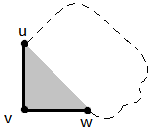
\includegraphics[height=5cm]{rysunki/triangulacja_1.png} \hspace{3cm} 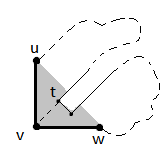
\includegraphics[height=5cm]{rysunki/triangulacja_2.png}
	\end{align*}
	\\\indent W pierwszym przypadku przekątna $\overline{u w}$ dzieli wielokąt na trójkąt oraz wielokąt prosty o $n - 1$ wierzchołkach, na których wykonujemy krok indukcyjny, otrzymując $1 + (n - 1) -2 = n - 2$ trókątów, najbliższych do $v$.
	\\\indent W przypadku drugim znajdujemy punkt $t$, który znajduje się najdalej od prostej $uw$, a następnie łączymy go z punktem $v$. Odcinek $\overline{v t}$ musi być przekątną, która dzieli wielokąt na dwa proste wielokąty o $m$ oraz $n - m + 2$ wierzchołkach, gdzie $3 \ge m \ge n-1$ na których wykonujemy krok indukcji: z założenia indukcyjnego, podział wielokąta skłąda się z $(m - 2) + ((n - m + 2) -2) = n - 2$ trójkątow.
\end{proof}

% %Załącznik…
% %
% %\chapter{Tytuł załącznika}
% %
% %Załącznik…

\begin{thebibliography}{99}
 \bibitem{orourke}
 J. \ O'Rourke.
 \newblock{Art gallery theorems and algorithms (1987)}

 \bibitem{chvatal} 
  V. \ Chv\'atal. 
  \newblock{A combinatorial theorem in plane geometry.}
  \newblock{{\em Journal of Combinatorial Theory} 18, str. 39-41 (1975).}

 \bibitem{guarding walls} 
  A. \ Laurentini.
  \newblock{Guarding the walls of an art gallery.} 
  \newblock{The Visual Computer (1999)}

 \bibitem{czyzowicz} 
 J. \ Czyzowicz, E. \ Rivera-Campo N. \ Santoro, J. \ Urrutia i J. \ Zaks. 
 \newblock{Guarding rectangular art galleries.} 
 \newblock{{\em Discrete Applied Math} str. 149–157 (1994).}

 \bibitem{illumination} 
 J. \ Urrutia. 
 \newblock{Art gallery and illumination problems (2004).}

 \bibitem{knadajniki} 
 B. \ Ballinger, N. \ Benbernou, P. \ Bose, M. \ Damian, E. \ Demaine, V. \ Dujmovi\`c, R. \ Flatland, F. \ Hurtado, J. \ Iacono, A. \ Lubiw, P. \ Morin, V. \ Sacristán, D. \ Souvaine i R. \ Uehara. 
 \newblock{Coverage with k-transmittes in the presence of obstacles (?).}

 \bibitem{poscig} 
 R. \ Dawes. 
 \newblock{Some pursuit - evasion problems on grid.}

 \bibitem{fisk} 
 S. \ Fisk. 
 \newblock{A short proof of Chv\'atal's watchman theorem.} 
 \newblock{{\em Journal of Combinatorial Theory} 24, str. 374 (1977).}

 \bibitem{tutte} 
 W. \ Tutte. 
 \newblock{The Factorization of Linear Graphs.} 
 \newblock{{\em Journal of the London Mathematical Society} 22, str. 107-111 (1947).}

 \bibitem{ntafos} 
 S. \ Ntafos. 
 \newblock{On gallery watchmen in grids}
 \newblock{{\em Information Processing Letters} 23(3), str. 99–102 (1986).}

 \bibitem{avis} 
 D. \ Avis i G. \ Toussaint.
 \newblock{An efficient algorithm for decomposing a polygon into star-shaped polygons.}
 \newblock{{\em Pattern Recognition} 13(6), str. 395-398 (1981).}

 \bibitem{euler} 
 R. \ Courant i H. \ Robbins.
 \newblock{What is Mathematics?: An Elementary Approach to Ideas and Methods, str. 239-240 (1978).}

 \bibitem{nishizeki} 
 T. \ Nishizeki.
 \newblock{Precise proofs of some lemmas in the paper “Lower bounds on the cardinality of the maximum matchings of planar graphs”.}
 \newblock{Carnegie-Mellon tech. report (1977).}

 \bibitem{sciany}  
 F. \ Hurtado, O. \ Serra i J. \ Urrutia. 
 \newblock{Hiding points in arrangements of segments.}
 \newblock{{\em Discrete Mathematics} 162, str. 187–197 (1996).}

 \bibitem{erdosszekeres}  
 P. \ Erdös, G. \ Szekeres.
 \newblock{Classic Papers in Combinatorics Modern Birkhäuser Classics.}
 \newblock{{\em A Combinatorial Problem in Geometry} str. 49-56 (1987).}

 \bibitem{fabilamonroy} 
 R. \ Fabila-Monroy, A. R. \ Vargas i J. \ Urrutia.
 \newblock{On modem illumination problems.}
 \newblock{XIII Encuentros de Geometria Computacional (2009).}

 \bibitem{borodin} 
 O.V. \ Borodin.
 \newblock{Solution of Ringel's problems on vertex-face coloring of plane graphs and coloring of 1-planar graphs.}
 \newblock{{\em Metody Diskretnogo Analiza} 41,  str. 12-26  (1984).}

 \bibitem{even} 
 S. \ Even.
 \newblock{Graph Algorithms.}
 \newblock{Computer Science Press, Potomac, MD. (1979).}

 \bibitem{garey} 
 M. \ Garey i D. \ Johnson.
\newblock{Computers and Intractability: A Guide to the Theory of NP-Completeness (1979).}

 \bibitem{sugiharu} 
 K. \ Sugihara, I. \ Suzuki.
 \newblock{On a pursuit-evasion problem related to motion coordination of mobile robots.}
 \newblock{Proc. 21~1 Hawuii  Internat.  Conf  on System  Sciences,  Kailua- Kona,  Hawaii  str. 218-226 (1988).}

 \bibitem{appel} 
 K. \ Appel, W. \ Haken.
 \newblock{Every planar map is four colorable.}
 \newblock{{\em Illinois J. Math} 21(3), str. 429-490 (1977).} 

 \bibitem{topp} 
 J. \ Topp. 
 \newblock{Algebra Liniowa.}
 \newblock{Politechnika Gdańska, str. 131 (2005).}
\end{thebibliography}

% spis rysunków
\listoffigures

\oswiadczenie

\end{document}